\documentclass{article}
\usepackage[preprint]{neurips_2026}

\usepackage[utf8]{inputenc}
\usepackage[T1]{fontenc}
\usepackage{hyperref}
\usepackage{url}
\usepackage{booktabs}
\usepackage{amsfonts}
\usepackage{amsmath}
\usepackage{microtype}
\usepackage{xcolor}
\usepackage{graphicx}
\hypersetup{hidelinks}

% This is an ES 678 course paper, not a conference submission.
\makeatletter
\renewcommand{\@noticestring}{ES 678 Course Project}
\makeatother

% Auto-generated by src/paper_numbers.py from results/ and history/; do not edit by hand.
\newcommand{\Ndupnames}{42}
\newcommand{\Nmajshare}{19.1}
\newcommand{\Nmajlabel}{Laying}
\newcommand{\Nsdmin}{0.04}
\newcommand{\Nsdmax}{0.75}
\newcommand{\Nngrav}{60}
\newcommand{\Nnkeep}{501}
\newcommand{\Nnlinks}{6,752}
\newcommand{\Nnpairs}{7,351}
\newcommand{\Nnseg}{600}
\newcommand{\Nseglenmed}{12}
\newcommand{\Nseglenmax}{29}
\newcommand{\Nsegperminsa}{4}
\newcommand{\Nsegpermedsa}{4}
\newcommand{\Nnseeds}{10}
\newcommand{\Nrfgaplargest}{10}
\newcommand{\NoverlapR}{93.6}
\newcommand{\NsaS}{99.4}
\newcommand{\Ngrpvalsubjmin}{4}
\newcommand{\Ngrpvalsubjmax}{5}
\newcommand{\NmfDummyP}{0.054}
\newcommand{\NmfsdDummyP}{0.000}
\newcommand{\NaccDummyP}{0.191}
\newcommand{\NbaDummyP}{0.167}
\newcommand{\NfsdDummyP}{0.002}
\newcommand{\NmfsdzDummyP}{.000}
\newcommand{\NfsdzDummyP}{.002}
\newcommand{\NmfDummyR}{0.054}
\newcommand{\NmfsdDummyR}{0.000}
\newcommand{\NaccDummyR}{0.191}
\newcommand{\NbaDummyR}{0.167}
\newcommand{\NfsdDummyR}{0.000}
\newcommand{\NmfsdzDummyR}{.000}
\newcommand{\NfsdzDummyR}{.000}
\newcommand{\NmfDummyS}{0.079}
\newcommand{\NmfsdDummyS}{0.005}
\newcommand{\NaccDummyS}{0.164}
\newcommand{\NbaDummyS}{0.144}
\newcommand{\NfsdDummyS}{0.006}
\newcommand{\NmfsdzDummyS}{.005}
\newcommand{\NfsdzDummyS}{.006}
\newcommand{\NmfLRP}{0.931}
\newcommand{\NmfsdLRP}{0.004}
\newcommand{\NaccLRP}{0.932}
\newcommand{\NbaLRP}{0.931}
\newcommand{\NfsdLRP}{0.035}
\newcommand{\NmfsdzLRP}{.004}
\newcommand{\NfsdzLRP}{.035}
\newcommand{\NmfLRR}{0.986}
\newcommand{\NmfsdLRR}{0.001}
\newcommand{\NaccLRR}{0.985}
\newcommand{\NbaLRR}{0.986}
\newcommand{\NfsdLRR}{0.002}
\newcommand{\NmfsdzLRR}{.001}
\newcommand{\NfsdzLRR}{.002}
\newcommand{\NmfLRS}{0.973}
\newcommand{\NmfsdLRS}{0.002}
\newcommand{\NaccLRS}{0.972}
\newcommand{\NbaLRS}{0.973}
\newcommand{\NfsdLRS}{0.010}
\newcommand{\NmfsdzLRS}{.002}
\newcommand{\NfsdzLRS}{.010}
\newcommand{\NmfRFP}{0.910}
\newcommand{\NmfsdRFP}{0.003}
\newcommand{\NaccRFP}{0.912}
\newcommand{\NbaRFP}{0.910}
\newcommand{\NfsdRFP}{0.038}
\newcommand{\NmfsdzRFP}{.003}
\newcommand{\NfsdzRFP}{.038}
\newcommand{\NmfRFR}{0.981}
\newcommand{\NmfsdRFR}{0.001}
\newcommand{\NaccRFR}{0.981}
\newcommand{\NbaRFR}{0.981}
\newcommand{\NfsdRFR}{0.003}
\newcommand{\NmfsdzRFR}{.001}
\newcommand{\NfsdzRFR}{.003}
\newcommand{\NmfRFS}{0.956}
\newcommand{\NmfsdRFS}{0.003}
\newcommand{\NaccRFS}{0.955}
\newcommand{\NbaRFS}{0.956}
\newcommand{\NfsdRFS}{0.017}
\newcommand{\NmfsdzRFS}{.003}
\newcommand{\NfsdzRFS}{.017}
\newcommand{\NmfSVMP}{0.924}
\newcommand{\NmfsdSVMP}{0.004}
\newcommand{\NaccSVMP}{0.925}
\newcommand{\NbaSVMP}{0.925}
\newcommand{\NfsdSVMP}{0.032}
\newcommand{\NmfsdzSVMP}{.004}
\newcommand{\NfsdzSVMP}{.032}
\newcommand{\NmfSVMR}{0.979}
\newcommand{\NmfsdSVMR}{0.000}
\newcommand{\NaccSVMR}{0.978}
\newcommand{\NbaSVMR}{0.979}
\newcommand{\NfsdSVMR}{0.003}
\newcommand{\NmfsdzSVMR}{.000}
\newcommand{\NfsdzSVMR}{.003}
\newcommand{\NmfSVMS}{0.966}
\newcommand{\NmfsdSVMS}{0.002}
\newcommand{\NaccSVMS}{0.965}
\newcommand{\NbaSVMS}{0.967}
\newcommand{\NfsdSVMS}{0.010}
\newcommand{\NmfsdzSVMS}{.002}
\newcommand{\NfsdzSVMS}{.010}
\newcommand{\NfsdRmax}{0.003}
\newcommand{\NfsdPmin}{0.032}
\newcommand{\NfsdPmax}{0.038}
\newcommand{\NseedsdPmax}{0.004}
\newcommand{\NgapLR}{0.055}
\newcommand{\NgapsdLR}{0.004}
\newcommand{\NgapminLR}{0.050}
\newcommand{\NgapmaxLR}{0.061}
\newcommand{\NgapRSLR}{0.012}
\newcommand{\NgapSPLR}{0.042}
\newcommand{\NgapposLR}{10}
\newcommand{\NgapSVM}{0.056}
\newcommand{\NgapsdSVM}{0.004}
\newcommand{\NgapminSVM}{0.050}
\newcommand{\NgapmaxSVM}{0.062}
\newcommand{\NgapRSSVM}{0.013}
\newcommand{\NgapSPSVM}{0.043}
\newcommand{\NgapposSVM}{10}
\newcommand{\NgapRF}{0.072}
\newcommand{\NgapsdRF}{0.003}
\newcommand{\NgapminRF}{0.067}
\newcommand{\NgapmaxRF}{0.076}
\newcommand{\NgapRSRF}{0.025}
\newcommand{\NgapSPRF}{0.047}
\newcommand{\NgapposRF}{10}
\newcommand{\Noverlapsharemin}{23}
\newcommand{\Noverlapsharemax}{35}
\newcommand{\Ngapmodelmin}{0.055}
\newcommand{\Ngapmodelmax}{0.072}
\newcommand{\Nrfexcess}{0.016}
\newcommand{\Noverlapshareseedmin}{18}
\newcommand{\Noverlapshareseedmax}{43}
\newcommand{\Ngapallmin}{0.050}
\newcommand{\Ngapallmax}{0.076}
\newcommand{\NdummySegLay}{31}
\newcommand{\NdummySegStand}{17}
\newcommand{\NdummySegOther}{2}
\newcommand{\NdummySegFolds}{50}
\newcommand{\Nstandshare}{18.7}
\newcommand{\Nnangle}{7}
\newcommand{\Nntgrav}{40}
\newcommand{\Nntgravmag}{13}
\newcommand{\Nnsingleseg}{1}
\newcommand{\Nfsdallmin}{0.010}
\newcommand{\NwinsLR}{10}
\newcommand{\NwinsSVM}{0}
\newcommand{\NwinsRF}{0}
\newcommand{\NdropLRWalk}{0.057}
\newcommand{\NdropLRUpstairs}{0.084}
\newcommand{\NdropLRDownstairs}{0.067}
\newcommand{\NdropLRSit}{0.054}
\newcommand{\NdropLRStand}{0.053}
\newcommand{\NdropLRLay}{0.013}
\newcommand{\NablLRMacrofull}{0.055}
\newcommand{\NablLRMacrong}{0.056}
\newcommand{\NablLRMacron}{4}
\newcommand{\NablLRMacroPfull}{0.931}
\newcommand{\NablLRMacroPng}{0.899}
\newcommand{\NablLRSitfull}{0.054}
\newcommand{\NablLRSitng}{0.041}
\newcommand{\NablLRSitn}{9}
\newcommand{\NablLRSitPfull}{0.904}
\newcommand{\NablLRSitPng}{0.853}
\newcommand{\NablLRStandfull}{0.053}
\newcommand{\NablLRStandng}{0.032}
\newcommand{\NablLRStandn}{10}
\newcommand{\NablLRStandPfull}{0.908}
\newcommand{\NablLRStandPng}{0.885}
\newcommand{\NablLRLayfull}{0.013}
\newcommand{\NablLRLayng}{0.043}
\newcommand{\NablLRLayn}{0}
\newcommand{\NablLRLayPfull}{0.987}
\newcommand{\NablLRLayPng}{0.882}
\newcommand{\NpermLRbase}{0.928}
\newcommand{\NpermLR}{0.629}
\newcommand{\NpermLRSit}{0.478}
\newcommand{\NablLRSitRfull}{0.958}
\newcommand{\NablLRSitRng}{0.894}
\newcommand{\NdropSVMWalk}{0.070}
\newcommand{\NdropSVMUpstairs}{0.085}
\newcommand{\NdropSVMDownstairs}{0.091}
\newcommand{\NdropSVMSit}{0.042}
\newcommand{\NdropSVMStand}{0.036}
\newcommand{\NdropSVMLay}{0.010}
\newcommand{\NablSVMMacrofull}{0.056}
\newcommand{\NablSVMMacrong}{0.069}
\newcommand{\NablSVMMacron}{0}
\newcommand{\NablSVMMacroPfull}{0.924}
\newcommand{\NablSVMMacroPng}{0.872}
\newcommand{\NablSVMSitfull}{0.042}
\newcommand{\NablSVMSitng}{0.057}
\newcommand{\NablSVMSitn}{0}
\newcommand{\NablSVMSitPfull}{0.899}
\newcommand{\NablSVMSitPng}{0.799}
\newcommand{\NablSVMStandfull}{0.036}
\newcommand{\NablSVMStandng}{0.036}
\newcommand{\NablSVMStandn}{6}
\newcommand{\NablSVMStandPfull}{0.910}
\newcommand{\NablSVMStandPng}{0.857}
\newcommand{\NablSVMLayfull}{0.010}
\newcommand{\NablSVMLayng}{0.050}
\newcommand{\NablSVMLayn}{0}
\newcommand{\NablSVMLayPfull}{0.988}
\newcommand{\NablSVMLayPng}{0.861}
\newcommand{\NpermSVMbase}{0.925}
\newcommand{\NpermSVM}{0.645}
\newcommand{\NpermSVMSit}{0.491}
\newcommand{\NablSVMSitRfull}{0.941}
\newcommand{\NablSVMSitRng}{0.856}
\newcommand{\NdropRFWalk}{0.072}
\newcommand{\NdropRFUpstairs}{0.113}
\newcommand{\NdropRFDownstairs}{0.084}
\newcommand{\NdropRFSit}{0.081}
\newcommand{\NdropRFStand}{0.073}
\newcommand{\NdropRFLay}{0.006}
\newcommand{\NablRFMacrofull}{0.072}
\newcommand{\NablRFMacrong}{0.067}
\newcommand{\NablRFMacron}{9}
\newcommand{\NablRFMacroPfull}{0.910}
\newcommand{\NablRFMacroPng}{0.878}
\newcommand{\NablRFSitfull}{0.081}
\newcommand{\NablRFSitng}{0.061}
\newcommand{\NablRFSitn}{10}
\newcommand{\NablRFSitPfull}{0.881}
\newcommand{\NablRFSitPng}{0.829}
\newcommand{\NablRFStandfull}{0.073}
\newcommand{\NablRFStandng}{0.046}
\newcommand{\NablRFStandn}{10}
\newcommand{\NablRFStandPfull}{0.892}
\newcommand{\NablRFStandPng}{0.852}
\newcommand{\NablRFLayfull}{0.006}
\newcommand{\NablRFLayng}{0.064}
\newcommand{\NablRFLayn}{0}
\newcommand{\NablRFLayPfull}{0.994}
\newcommand{\NablRFLayPng}{0.868}
\newcommand{\NpermRFbase}{0.909}
\newcommand{\NpermRF}{0.564}
\newcommand{\NpermRFSit}{0.414}
\newcommand{\NablRFSitRfull}{0.962}
\newcommand{\NablRFSitRng}{0.891}
\newcommand{\Nnperm}{10}
\newcommand{\Ntestsharemin}{14}
\newcommand{\Ntestsharemax}{18}
\newcommand{\NtuneLR}{0.927}
\newcommand{\NtunesdLR}{0.037}
\newcommand{\NtuneSVM}{0.931}
\newcommand{\NtunesdSVM}{0.025}
\newcommand{\NtuneRF}{0.926}
\newcommand{\NtunesdRF}{0.030}
\newcommand{\NtuneLRC}{10}
\newcommand{\NtuneSVMC}{100}
\newcommand{\NtuneSVMgamma}{0.0005}
\newcommand{\NtuneRFtrees}{500}
\newcommand{\NtuneRFmf}{$\log_2 d$}
\newcommand{\NtuneRFleaf}{1}
\newcommand{\Nselmodel}{SVM}
\newcommand{\Nselcv}{0.931}
\newcommand{\Nselcvsd}{0.025}
\newcommand{\Nselmargin}{0.004}
\newcommand{\Nselboundary}{none}
\newcommand{\NtuneRFboundary}{max\_features, min\_samples\_leaf, n\_estimators}
\newcommand{\NtuneRFone}{0.908}
\newcommand{\NtuneRFoneleaf}{4}
\newcommand{\NtuneRFn}{26}
\newcommand{\Nsmoketestf}{0.955}
\newcommand{\NsmokeC}{1}
\newcommand{\Nrunonetestf}{0.952}
\newcommand{\NrunoneC}{10}
\newcommand{\Ntestf}{0.961}
\newcommand{\Ntestacc}{0.961}
\newcommand{\Ntestbal}{0.960}
\newcommand{\Ntestminuscv}{+0.029}
\newcommand{\Ntestcorrect}{2,833}
\newcommand{\Ntesttotal}{2,947}
\newcommand{\Nsubjmin}{0.907}
\newcommand{\Nsubjmed}{0.968}
\newcommand{\Nsubjmax}{0.995}
\newcommand{\Nsubjminid}{10}
\newcommand{\Nnerr}{114}
\newcommand{\Nnwithinstatic}{62}
\newcommand{\Nnwithindyn}{51}
\newcommand{\Nncross}{1}
\newcommand{\NconfAn}{48}
\newcommand{\NconfApct}{9.8}
\newcommand{\NconfBn}{22}
\newcommand{\NconfBpct}{5.2}
\newcommand{\NconfCn}{15}
\newcommand{\NconfCpct}{3.2}
\newcommand{\NtestprecWalk}{0.959}
\newcommand{\NtestrecWalk}{0.986}
\newcommand{\NtestfoneWalk}{0.972}
\newcommand{\NtestprecUpstairs}{0.944}
\newcommand{\NtestrecUpstairs}{0.966}
\newcommand{\NtestfoneUpstairs}{0.955}
\newcommand{\NtestprecDownstairs}{0.990}
\newcommand{\NtestrecDownstairs}{0.933}
\newcommand{\NtestfoneDownstairs}{0.961}
\newcommand{\NtestprecSit}{0.969}
\newcommand{\NtestrecSit}{0.900}
\newcommand{\NtestfoneSit}{0.933}
\newcommand{\NtestprecStand}{0.915}
\newcommand{\NtestrecStand}{0.974}
\newcommand{\NtestfoneStand}{0.944}
\newcommand{\NtestprecLay}{1.000}
\newcommand{\NtestrecLay}{1.000}
\newcommand{\NtestfoneLay}{1.000}
\newcommand{\Npyver}{3.13.18}
\newcommand{\Nsklearn}{1.6.1}
\newcommand{\Nncpu}{4}
\newcommand{\Nrunhours}{2.2}


\title{How Validation Strategy Affects Generalization in\\Smartphone-Based Human Activity Recognition}

\author{%
  [STUDENT NAME] \\
  Roll Number: [ROLL NUMBER] \\
  ES 678 \\
  Indian Institute of Technology Gandhinagar
}

\begin{document}
\maketitle

\begin{abstract}
Smartphone activity-recognition models are used on new people but are often validated by randomly splitting overlapping sensor windows. On the UCI HAR training partition (21 participants) we compare fixed logistic regression, RBF SVM and random forest models under three 5-fold protocols, each repeated over \Nnseeds{} split seeds: random-window CV, participant-grouped CV, and segment-grouped CV, which keeps exactly reconstructed chains of overlapping windows together. Random-window CV gave higher macro-F1 than participant-grouped CV for every model and seed, by \Ngapmodelmin--\Ngapmodelmax{} on average. Segment-grouped CV fell in between; descriptively, it accounted for \Noverlapsharemin--\Noverlapsharemax\% of the difference, and the remainder is associated with participant separation and other within-participant dependencies. The gap differed between activities. Gravity-feature ablation and permutation showed that these features are predictive but did not identify a mechanism.
\end{abstract}

\section{Introduction}
Activity-recognition models are used by new people, so what matters is performance on \emph{unseen participants}. Random window-level cross-validation (CV) puts every participant in both training and validation folds, and since UCI HAR windows overlap by 50\%, a validation window can share half its raw samples with a training window. The problem is known. \citet{saeb2017} showed that record-wise splits overestimate subject-wise accuracy in clinical sensor studies. \citet{dehghani2019} compared $k$-fold and subject CV on a 17-subject dataset of 33 fitness activities recorded with nine body-worn IMUs; $k$-fold CV raised performance by about 10\%, and by 16\% with overlapping windows. \citet{braganca2022} merged three smartphone datasets including UCI HAR (59 subjects) and found $k$-fold accuracy of 98\% against 85.37\% under leave-one-subject-out validation, using SHAP to inspect features. \citet{rehman2024} reported a similar gap on PAMAP2 (89\% vs.\ 76\% for a random forest). We claim no new phenomenon; we contribute a controlled audit of the UCI HAR training split that uses exactly reconstructed overlap chains to separate direct window overlap from other dependencies, asking: (RQ1) how large and stable is random-window optimism; (RQ2) where does segment-grouped CV fall; (RQ3) which activities carry the gap, and what do gravity-feature diagnostics support?

\section{Data and Preparation}
UCI HAR \citep{anguita2013,uci_har} (CC BY 4.0) has 10,299 windows from 30 volunteers who wore a smartphone on the waist and performed six scripted activities (walking, walking upstairs, walking downstairs, sitting, standing, laying). Signals at 50\,Hz were cut into 2.56\,s windows (128 samples, 50\% overlap) described by 561 engineered features. The official split has 7,352 training windows from 21 participants and 2,947 test windows from nine others. An audit confirms counts, row alignment of features, labels, IDs and raw signals, disjoint train/test participants, and no missing, infinite, constant or duplicate values. Participant IDs only define folds. Classes are near balanced (largest: \Nmajlabel, \Nmajshare\%). LR and the SVM standardise features in a scikit-learn pipeline \citep{sklearn} fitted on training folds only.

\section{Methods and Evaluation Design}
\textbf{Models.} A majority-class baseline, logistic regression (LR), an RBF SVM and a random forest (RF), each with a configuration fixed in advance for the protocol comparison: LR $C{=}1$; SVM $C{=}1$, $\gamma{=}$\texttt{scale}; RF 400 trees, $\sqrt{561}$ features per split, leaf size 1.

\textbf{Validation protocols.} All use the 7,352 training windows, five folds and split seeds 42--51. \emph{Random-window CV} (\texttt{StratifiedKFold}) lets participants and overlapping neighbours appear on both sides. \emph{Participant-grouped CV} (\texttt{StratifiedGroupKFold}, participant groups) keeps each person in one fold of \Ngrpvalsubjmin--\Ngrpvalsubjmax{} people. \emph{Segment-grouped CV} uses the same splitter with segment groups. For \Nnlinks{} of \Nnpairs{} consecutive rows of the raw \texttt{Inertial Signals}, the last 64 samples of one window equal the first 64 of the next exactly (tolerance 0) on all nine channels. Every match lies within one participant and activity, and no non-adjacent pair matches; maximal chains form \Nnseg{} segments (median \Nseglenmed{} windows; \Nnsingleseg{} single-window segment). Every fold is checked for disjoint groups and all six classes. In random-window folds \NoverlapR\% of validation windows have an overlapping neighbour in training; segment grouping removes all shared samples, yet \NsaS\% of its validation windows still have training windows from the same participant and activity.

\textbf{Metrics and variability.} Macro-F1 is primary because it weights activities equally; accuracy and balanced accuracy (BA, mean per-class recall) are supplementary. For each seed we pool the five folds' out-of-fold predictions and compute each metric once. The \emph{across-seed SD} of these ten values reflects the fold assignment; the \emph{within-seed fold SD} (over one seed's five validation folds, averaged over seeds) reflects variation between held-out groups. The \emph{gap} is random-window minus participant-grouped macro-F1, paired by seed. Seeds reuse the same 21 people, so neither SD is a confidence interval.

\textbf{Gravity diagnostics.} The gravity family is the \Nngrav{} features whose names contain ``gravity'' (\Nntgrav{} \texttt{tGravityAcc}, \Nntgravmag{} \texttt{tGravityAccMag}, all \Nnangle{} \texttt{angle}). \emph{Ablation} retrains the fixed models on the other \Nnkeep{} features with the same folds and seeds. \emph{Joint permutation} shuffles the rows of the whole block inside each held-out fold of the fitted models (seed 42, \Nnperm{} permutations, all three models).

\textbf{Model selection.} A separate grid search used participant-grouped CV (seed 42) and macro-F1: LR $C\in\{0.01,\dots,100\}$; SVM $C\in\{0.1,\dots,1000\}\times\gamma\in\{10^{-4},5{\cdot}10^{-4},\texttt{scale},0.005,0.01\}$ (extended once after a smaller grid peaked at a corner); RF trees $\in\{300,500\}$, features $\in\{\sqrt{d},0.5d\}$, leaf $\in\{1,2,4\}$, plus one bounded extension (\S\ref{sec:select}). The best family is selected.

\section{Results and Validation-Optimism Analysis}
\begin{table}[t]
\centering
\caption{Fixed configurations on the training partition: means over \Nnseeds{} split seeds of pooled out-of-fold scores; s = across-seed SD, f = within-seed fold SD of macro-F1.}
\label{tab:main}
\footnotesize
\setlength{\tabcolsep}{2.25pt}
\begin{tabular}{l ccccc ccccc ccccc}
\toprule
& \multicolumn{5}{c}{Random-window CV} & \multicolumn{5}{c}{Segment-grouped CV} & \multicolumn{5}{c}{Participant-grouped CV} \\
\cmidrule(lr){2-6}\cmidrule(lr){7-11}\cmidrule(lr){12-16}
Model & Macro-F1 & s & f & Acc. & BA & Macro-F1 & s & f & Acc. & BA & Macro-F1 & s & f & Acc. & BA \\
\midrule
Majority & \NmfDummyR & \NmfsdzDummyR & \NfsdzDummyR & \NaccDummyR & \NbaDummyR & \NmfDummyS & \NmfsdzDummyS & \NfsdzDummyS & \NaccDummyS & \NbaDummyS & \NmfDummyP & \NmfsdzDummyP & \NfsdzDummyP & \NaccDummyP & \NbaDummyP \\
LR & \NmfLRR & \NmfsdzLRR & \NfsdzLRR & \NaccLRR & \NbaLRR & \NmfLRS & \NmfsdzLRS & \NfsdzLRS & \NaccLRS & \NbaLRS & \NmfLRP & \NmfsdzLRP & \NfsdzLRP & \NaccLRP & \NbaLRP \\
RBF SVM & \NmfSVMR & \NmfsdzSVMR & \NfsdzSVMR & \NaccSVMR & \NbaSVMR & \NmfSVMS & \NmfsdzSVMS & \NfsdzSVMS & \NaccSVMS & \NbaSVMS & \NmfSVMP & \NmfsdzSVMP & \NfsdzSVMP & \NaccSVMP & \NbaSVMP \\
RF & \NmfRFR & \NmfsdzRFR & \NfsdzRFR & \NaccRFR & \NbaRFR & \NmfRFS & \NmfsdzRFS & \NfsdzRFS & \NaccRFS & \NbaRFS & \NmfRFP & \NmfsdzRFP & \NfsdzRFP & \NaccRFP & \NbaRFP \\
\bottomrule
\end{tabular}
\end{table}

\subsection{Validation-protocol comparison (RQ1--RQ2)}
\textbf{Size and stability of the gap.} Random-window CV gave higher macro-F1 than participant-grouped CV for all three models in all \Nnseeds{} seeds (Table~\ref{tab:main}); accuracy and BA agree. The paired gap is \NgapLR{} for LR (per-seed range \NgapminLR--\NgapmaxLR), \NgapSVM{} for the SVM (\NgapminSVM--\NgapmaxSVM) and \NgapRF{} for RF (\NgapminRF--\NgapmaxRF). The across-seed SD is at most \NseedsdPmax, so no single split drives the result, but held-out groups differ much more: participant-grouped folds have a within-seed fold SD of \NfsdPmin--\NfsdPmax, against at most \NfsdRmax{} for random-window folds. Random-window CV thus overstates performance on new people and understates its variability.

\textbf{What segment grouping removes.} Segment-grouped CV lies between the other two for every model. Keeping overlap chains together lowers macro-F1 by \NgapRSLR{} (LR), \NgapRSSVM{} (SVM) and \NgapRSRF{} (RF); separating participants lowers it by a further \NgapSPLR, \NgapSPSVM{} and \NgapSPRF. As a descriptive, protocol-based decomposition, segment grouping accounts for \Noverlapsharemin--\Noverlapsharemax\% of the mean gap (\Noverlapshareseedmin--\Noverlapshareseedmax\% across seeds; computed before rounding). This is not a causal attribution: segment grouping removes only direct sample overlap, and most of its validation windows keep same-participant, same-activity (usually same-session) windows in training. The remaining difference is thus associated with participant separation \emph{together with} session, temporal-proximity and fold-composition effects.

\textbf{Model differences and the baseline.} LR had the best grouped macro-F1 in \NwinsLR{} of \Nnseeds{} seeds, and RF the largest gap in \Nrfgaplargest{} seeds (\Nrfexcess{} above the next on average). Both are small relative to the fold SD, so they are observed patterns, not model properties. The majority baseline predicts one class per fold, so five classes get F1\,=\,0; under random-window and participant-grouped CV it always predicts laying (accuracy = laying share, BA $=1/6$). Laying and standing (\Nstandshare\%) have similar shares, so under segment grouping the training-fold majority varies (laying in \NdummySegLay{} of \NdummySegFolds{} folds, standing in \NdummySegStand, other \NdummySegOther) and pooled predictions mix classes.

\begin{figure}[t]
\centering
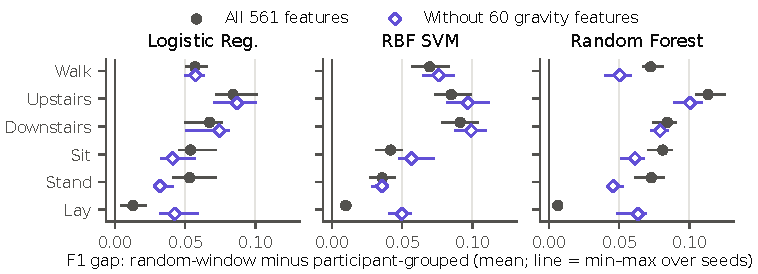
\includegraphics[width=\linewidth]{figures/per_class_drop_ablation.pdf}
\caption{Per-class F1 gap, random-window minus participant-grouped CV, with all features (filled) and without the \Nngrav{} gravity features (open). Markers: mean over \Nnseeds{} seeds; lines: min--max over seeds.}
\label{fig:ablation}
\end{figure}

\subsection{Activity-wise and feature diagnostics (RQ3)}
The gap is not uniform across activities (Fig.~\ref{fig:ablation}). Among moving activities, walking upstairs has the largest gap (LR \NdropLRUpstairs, SVM \NdropSVMUpstairs, RF \NdropRFUpstairs); sitting and standing have gaps of \NdropSVMStand--\NdropRFSit, while laying barely changes (at most \NdropLRLay).
Removing the gravity family lowered grouped macro-F1 for every model (LR \NablLRMacroPfull{}\,$\to$\,\NablLRMacroPng, SVM \NablSVMMacroPfull{}\,$\to$\,\NablSVMMacroPng, RF \NablRFMacroPfull{}\,$\to$\,\NablRFMacroPng), so these features carry useful predictive information. The overall gap did not shrink (LR \NablLRMacrofull{}\,$\to$\,\NablLRMacrong, SVM \NablSVMMacrofull{}\,$\to$\,\NablSVMMacrong, RF \NablRFMacrofull{}\,$\to$\,\NablRFMacrong), and class gaps moved in different directions: sitting and standing gaps narrowed for LR and RF, mainly because random-window scores fell (LR random-window sitting F1 \NablLRSitRfull{}\,$\to$\,\NablLRSitRng), whereas the SVM's sitting gap and every model's laying gap widened. Jointly permuting the block in held-out grouped folds lowered macro-F1 from \NpermLRbase{} to \NpermLR{} (LR), \NpermSVMbase{} to \NpermSVM{} (SVM) and \NpermRFbase{} to \NpermRF{} (RF). The models are sensitive to disruption of the block, but permutation breaks its correlation with other features and creates unrealistic inputs, so it does not measure causal importance; neither diagnostic shows that gravity features encode participant identity, body geometry or phone orientation.

\subsection{Model selection and supplementary test-partition result}
\label{sec:select}
Model selection is a separate experiment from Table~\ref{tab:main}. The best grouped-CV scores were \NtuneLR{} for LR ($C{=}\NtuneLRC$), \NtuneSVM{} for the SVM ($C{=}\NtuneSVMC$, $\gamma{=}\NtuneSVMgamma$, inside the grid) and \NtuneRF{} for RF. The RF's first grid peaked at the leaf-size edge (\NtuneRFone, leaf \NtuneRFoneleaf); one bounded extension ($\log_2 d$ features with leaf $\in\{1,\dots,16\}$; $\sqrt{d}$ with leaf $\in\{8,16\}$; \NtuneRFn{} settings in all) moved the best to \NtuneRFtrees{} trees, \NtuneRFmf{} features, leaf \NtuneRFleaf. This is still at the edge of the explored feature-subset and tree ranges, so the RF result is provisional; we did not extend again. The \Nselmodel{} was selected (\Nselcv, fold SD \Nselcvsd), but its margin over LR (\Nselmargin) is far below the fold SD: a narrow numerical preference, not evidence of superiority. Table~\ref{tab:main}, where LR led, compares \emph{fixed} configurations, so the two do not conflict.

\textbf{Supplementary test-partition result.} The official test partition was evaluated during earlier development (\S\ref{sec:repro}), so it is not an untouched holdout; we report it only as a descriptive check, not used for selection and not an independent estimate of generalization. Refitted on all training windows, the SVM reached macro-F1 \Ntestf, accuracy \Ntestacc{} and BA \Ntestbal{} on the nine test participants (per-participant macro-F1 \Nsubjmin--\Nsubjmax). Sitting predicted as standing was the main error (\NconfAn{} of \Nnerr). Earlier LR test scores (\Nsmoketestf, \Nrunonetestf) differ from this by less than one grouped fold SD, so the test scores do not rank the models.

\section{Limitations and Conclusion}
With 21 development participants, grouped folds hold four or five people and all spreads are descriptive. Activities were scripted, with one waist-worn phone and the supplied features only. Tuning used one grouped split, and we did not run leave-one-subject-out CV. \emph{Conclusion.} On the UCI HAR training partition, random-window CV exceeded participant-grouped macro-F1 by \Ngapmodelmin--\Ngapmodelmax{} on average, in every split and for every model, and understated fold-to-fold variability. Direct window overlap accounts for part of this difference under our split design; the rest is associated with participant and session dependencies. Models for new users should be validated with participant-grouped splits.

\section{Reproducibility, Test-Set Access and AI Use}
\label{sec:repro}
\textbf{Code:} [REPOSITORY URL]. \texttt{scripts/run\_all.sh} runs every development step on the training partition only; \texttt{scripts/run\_final\_test.sh} is a separate, guarded test stage. Development ran on Kaggle CPU kernels (\Nncpu{} vCPUs, Python \Npyver, scikit-learn \Nsklearn).
\textbf{Test-set access.} The official test partition has been scored three times: a local pipeline smoke test (LR, $C{=}\NsmokeC$; macro-F1 \Nsmoketestf), the first full run reported in our first draft (LR, $C{=}\NrunoneC$; \Nrunonetestf), and the \Nselmodel{} above. In between we added segment-grouped CV and the gravity diagnostics and widened the SVM grid, and the selection changed from LR to SVM; AI critiques of the first draft and the grid-boundary rule prompted these changes, not test scores, but as earlier scores had been seen, independence cannot be demonstrated. Code hashes document provenance but do not restore a blind holdout. The later RF extension used the training partition only and did not change the selection; the test partition was not scored again.
\textbf{AI use:} Claude Code (Anthropic, Claude Opus 5.5) wrote the code, ran the experiments, made the figures, and drafted and revised this paper from the student's project brief and revision notes, which drew on AI critiques of earlier drafts ([STUDENT: name the tools and model versions]); these were AI feedback, not peer review. [STUDENT: state truthfully which code, results and claims you inspected, reran, corrected or rewrote yourself.]

{\footnotesize\setlength{\bibsep}{1pt}
\begin{thebibliography}{7}
\bibitem[Anguita et~al.(2013)]{anguita2013}
D.~Anguita, A.~Ghio, L.~Oneto, X.~Parra, and J.~L. Reyes-Ortiz.
\newblock A public domain dataset for human activity recognition using smartphones.
\newblock In \emph{Proc.\ ESANN}, pages 437--442, 2013.

\bibitem[Bragan{\c{c}}a et~al.(2022)]{braganca2022}
H.~Bragan{\c{c}}a, J.~G. Colonna, H.~A.~B.~F. Oliveira, and E.~Souto.
\newblock How validation methodology influences human activity recognition mobile systems.
\newblock \emph{Sensors}, 22(6):2360, 2022. doi:\nolinkurl{10.3390/s22062360}.

\bibitem[Dehghani et~al.(2019)]{dehghani2019}
A.~Dehghani, T.~Glatard, and E.~Shihab.
\newblock Subject cross validation in human activity recognition.
\newblock arXiv:1904.02666, 2019.

\bibitem[Pedregosa et~al.(2011)]{sklearn}
F.~Pedregosa, G.~Varoquaux, A.~Gramfort, V.~Michel, B.~Thirion, et~al.
\newblock Scikit-learn: Machine learning in {P}ython.
\newblock \emph{Journal of Machine Learning Research}, 12:2825--2830, 2011.

\bibitem[Rehman et~al.(2024)]{rehman2024}
S.~U. Rehman, A.~Ali, A.~M. Khan, and C.~Okpala.
\newblock Human activity recognition: A comparative study of validation methods and impact of feature extraction in wearable sensors.
\newblock \emph{Algorithms}, 17(12):556, 2024. doi:\nolinkurl{10.3390/a17120556}.

\bibitem[Reyes-Ortiz et~al.(2013)]{uci_har}
J.~Reyes-Ortiz, D.~Anguita, A.~Ghio, L.~Oneto, and X.~Parra.
\newblock Human activity recognition using smartphones.
\newblock UCI Machine Learning Repository, 2013. doi:\nolinkurl{10.24432/C54S4K}.

\bibitem[Saeb et~al.(2017)]{saeb2017}
S.~Saeb, L.~Lonini, A.~Jayaraman, D.~C. Mohr, and K.~P. Kording.
\newblock The need to approximate the use-case in clinical machine learning.
\newblock \emph{GigaScience}, 6(5):gix019, 2017. doi:\nolinkurl{10.1093/gigascience/gix019}.
\end{thebibliography}
}

\end{document}
